\chapter{Klassifikation}

Die Klassifikation besch\"aftigt sich mit der Einordnung von Objekten zu bestimmten Klassen. Die Objekte werden dabei durch einen sogenannten Merkmalsvektor \( x \in \mathbb{R}^n \) beschrieben, welcher definierte Eigenschaften des Objekts enth\"alt. Die benutzten Merkmale k\"onnen je nach Anwendungsfall unterschiedlich ausfallen. Im Bereich der Klassifikation von Verkehrsteilnehmern bieten sich geometrische Eigenschaften wie Ausma\ss{}e des Objekts, Umfang, Volumen oder Dichte an. Die zuzuordnende Klasse oder auch Label genannt ist im Allgemeinen eine ganze Zahl \(y \in \mathbb{Z} \). Der Klassifikator \(f\) l\"asst sich somit beschreiben als:

\begin{equation*}
 f: x \in \mathbb{R}^n \mapsto y \in \mathbb{Z}
\end{equation*}

Er ordnet den Merkmalen eines Objekts eine Klasse zu. Die Form des Klassifikators kann dabei variieren und h\"angt vom Anwendungsfall ab.
F\"ur gew\"ohnlich muss ein Klassifikator trainiert werden. Unter dem Begriff Training versteht man in diesem Zusammenhang den Vorgang, die w\"ahlbaren Parameter der Klassifikationsfunktion so einzustellen, dass er auf einen bestimmten Trainingsdatensatz \( (x_i | y_i)_{i=1..n} \) m\"oglichst gute Daten liefert. Das Training kann als Optimierungsproblem dargestellt werden:
\begin{equation*}
 \min_{\alpha} \sum_{i=1}^n \omega ( f_{\alpha}(x_i), y_i)
\end{equation*}
Die Funktion \( \omega : \mathbb{Z}^2 \mapsto \mathbb{R} \) ist eine Fehlerfunktion welche testet, ob die zu testende Klasse mit der vom Klassifikator ausgewerteten Klasse \"ubereinstimmt:
\begin{equation*}
 \omega (y_1, y_2) = 
 \begin{cases}
  0 & y_1=y_2 \\
  d(y_1, y_2) & y_1 \neq y_2, d>0
 \end{cases}
\end{equation*}

Durch Minimierung der Summe der Fehler kann so eine bestm\"ogliche Approximation an die Trainingsdaten gefunden werden. Im Folgenden werden einige Klassifikatoinsverfahren vorgestellt.

\section{K-Nearest-Neighbor Klassifikation}
Der Nearest-Neighbor-Klassifikator arbeitet ohne einen Optimiegunssprozess direkt auf den Trainingsdaten \( (x_i | y_i)_{i=1..m} \in \mathbb{R}^n \times \mathbb{Z} \). Ein Objekt mit Merkmalen \(b \in \mathbb{R}^n\) wird derjenigen Klasse zugeordnet, zu der der Abstand \(d=\|b-x_i\| \) am geringsten ist:
\begin{equation*}
 f(b)= y_k, k=\underset{{k \in \{1..m\}}}{arg\,min} (||b-x_k||)
\end{equation*}

Die Norm \(\| \cdot \| \) ist hierbei beliebig, h\"aufig wird jedoch die euklidische Norm \(\| \cdot \|_2 \) verwendet.

In Abbildung \ref{fig:classification_knn} ist ein Beispiel f\"ur eine solche Klassifikation zu sehen. Auf der linken Seite wird ein einfacher Nearest-Neighbor-Klassifikator angewendet. Auf der rechten Seite ist jedoch sichtbar, dass das Rauschen in den Daten zu einer Fehlklassifikation f\"uhren w\"urde. Aus diesem Grund wurde der Klassifikator erweitert zum K-Nearest-Neighbor-Klassifikator. Dieser bezieht nicht nur das Trainingsdatum mit dem geringsten Abstand ein, sondern sucht die \(k\) n\"achsten Nachbarn. Das Ergebnis der Klassifikation ist dann diejenige Klasse, welche am h\"aufigsten in dieser Ergebnismenge vorkommt. In der Grafik ist der KNN-Klassifikator f\"ur den fall \(k=3\) dargestellt.

Der KNN-Klassifikator finden h\"aufig zu Testzwecken Anwendung, da er einfach zu implementieren ist und stabile Resultate liefert. Da er kein Training ben\"otigt ist jedoch der Aufwand zur Evaluation hoch und der Algorithmus ist damit nicht sehr effizient. Zu produktiven Zwecken in Echtzeitsystemen wird er daher nur selten verwendet.

\begin{figure}
 \centering
 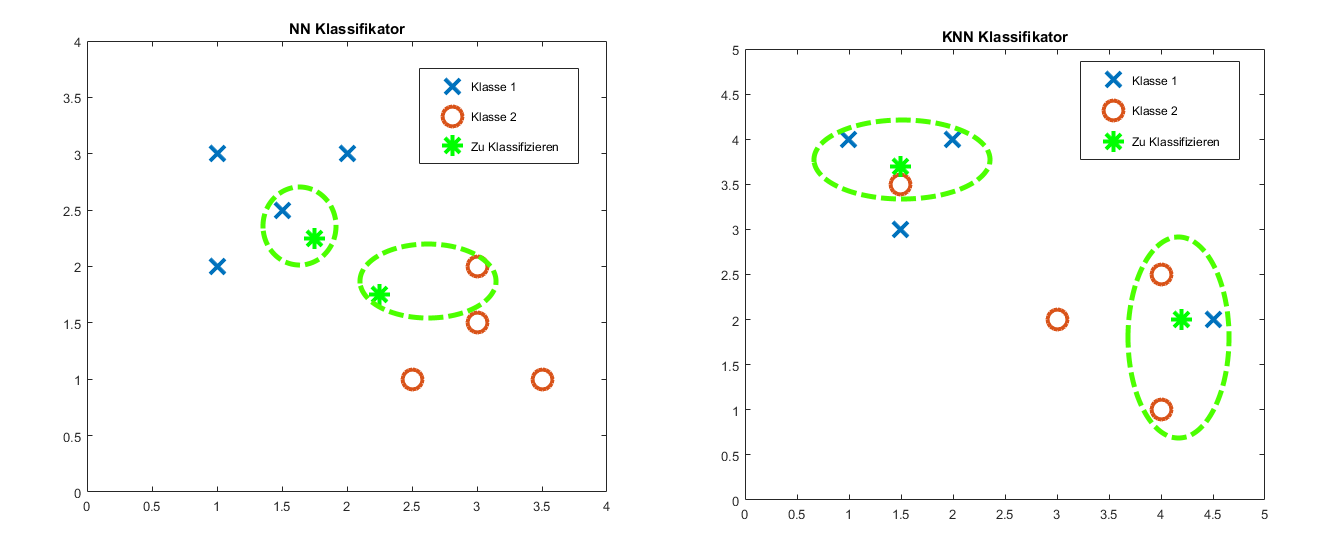
\includegraphics[width=1\textwidth]{media/classification/knn_example.png}
 \caption{Klassifikation - Beispiel f\"ur NN- und KNN-Klassifikator}
 \label{fig:classification_knn}
\end{figure}

\section{Logistische Regression}
Bin\"are Klassifikation
\begin{eqnarray*}
 h_{\beta}(x)=\frac{1}{1+e^{- (\beta_0+ \sum_{k=1}^m \beta_k x_{k}) }} \\
 f_{\beta}(x)= 
 \begin{cases}
  1 & h_{\beta}(x) \geq 0.5 \\
  0 & h_{\beta}(x) < 0.5
 \end{cases}
\end{eqnarray*}



\section{Support Vector Machine}
Die Klassifikation durch die sogenannte Support Vector Machine wird vorallem f\"ur bin\"are Klassifikationsprobleme verwendet. Ziel der Methode ist es, eine Hyperebene zu finden, welche zwei linear trennbare Mengen voneinander trennt. Der Klassifikator hat die Form
\begin{equation*}
 f_{w, b}(x) = 
 \begin{cases}
  1 & w^\intercal x+b>0 \\
  0 & sonst
 \end{cases}
\end{equation*}
 Der Vektor \(w \in \mathbb{R}^n \) ist die Normale der Ebene, das Skalar \(b \in \mathbb{R}\) ist der sogenannte Bias, also die Verschiebung. Diese beiden Parameter m\"ussen durch das Training des Klassifikators berechnet werden. Hierzu wird das Optimierungsproblem anhand der Trainingsdaten \( (x_i | y_i)_{i=1..m} \in \mathbb{R}^n \times \mathbb{Z} \) formuliert:
\begin{eqnarray*}
 & \min \frac{1}{2}||w||_2^2 \\
 & y_i(w^\intercal x_i+b) \geq 1, \forall (x_i | y_i)
\end{eqnarray*}
Die Nebenbedingung fordert hierbei, dass beide Klassen tats\"achlich linear trennbar sind. Da dies im Allgemeinen nicht der Fall ist wird eine sogenannte Schlupfvariable eingef\"ugt, welche die Verletzung der Nebenbedingung erlaubt:
\begin{eqnarray*}
 &\min \frac{1}{2}||w||_2^2+C \sum_{i=1}^m \xi_i \\
 &y_i(w^\intercal x_i+b) \geq 1-\xi_i, \forall (x_i | y_i)
\end{eqnarray*}

In Abbildung \ref{fig:classification_svmlinear} ist eine lineare Trennebene zu sehen. Die Methode der Support Vector Machine erm\"oglicht neben einer linearen auch eine nichtlineare Trennebene, was in Abbildung \ref{fig:classification_svmnonlinear} zu sehen ist. Das Optimierungsproblem gestaltet sich dabei deutlich komplexer, weshalb in der Arbeit auf die lineare Variante zur\"uckgegriffen wird.

\begin{figure}
\centering
\begin{minipage}{.5\textwidth}
  \centering
  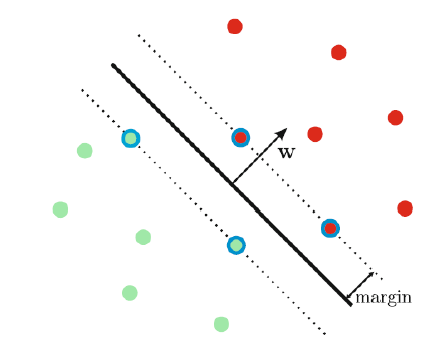
\includegraphics[width=1\textwidth]{media/classification/svm_linear.png}
  \captionof{figure}{SVM linear}
  \label{fig:classification_svmlinear}
\end{minipage}%
\begin{minipage}{.5\textwidth}
  \centering
  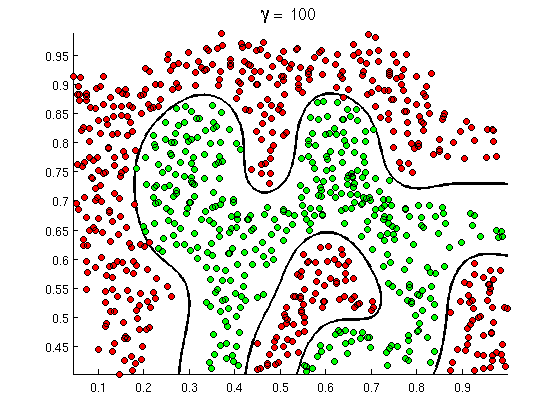
\includegraphics[width=1\textwidth]{media/classification/svm_nonlinear.png}
  \captionof{figure}{SVM nichtlinear}
  \label{fig:classification_svmnonlinear}
\end{minipage}
\end{figure}
